\documentclass[10pt]{article} % Changed to article document class
\usepackage{tikz}
\usetikzlibrary{positioning,calc}
\usepackage{graphicx} % Added graphicx package for figures
\usepackage{amsmath} % Added for align environment for equations
\usepackage{cancel} % Added for the \cancel command
\usepackage{hyperref} % For clickable links in the index
\hypersetup{
    colorlinks=true,
    linkcolor=black,
    urlcolor=blue,
    citecolor=black
}
\usepackage{tocloft} % For customizing the table of contents

% Add title and author information
\title{Fourier Series \& Transformation}
\author{Kirkwood Donavin -- Data Scientist}
\date{} % Suppress date

\begin{document}

% Display the title and author
\maketitle

\begin{center}
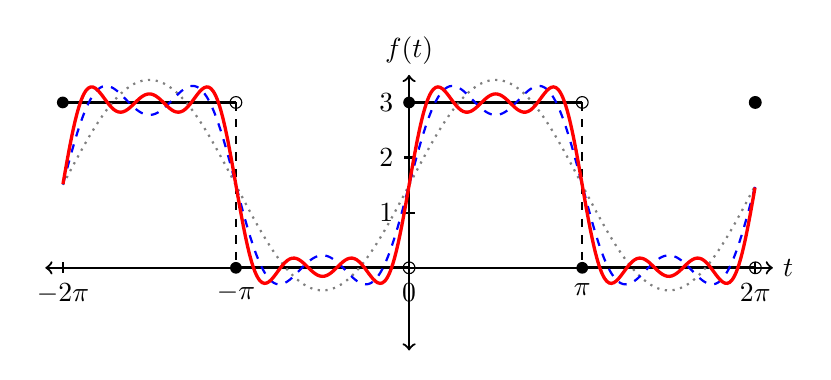
\begin{tikzpicture}[
    scale=0.7,
    solid_point/.style={circle,fill,inner sep=1.5pt},
    open_point/.style={circle,draw,inner sep=1.5pt}
]

% Axes
\draw[<->,thick] (-6.6,0) -- (6.6,0) node[right] {$t$};
\draw[<->,thick] (0,-1.5) -- (0,3.5) node[above] {$f(t)$};

% x-ticks at -2pi, -pi, 0, pi, 2pi
\foreach \i/\label in {-6.28/-2\pi, -3.14/-\pi, 0/0, 3.14/\pi, 6.28/2\pi}
    \draw[thick] (\i,0.1) -- (\i,-0.1) node[below] {$\label$};

% y-ticks at 1, 2, 3
\foreach \y in {1,2,3}
    \draw[thick] (0.1,\y) -- (-0.1,\y) node[left] {$\y$};

% Step function: f(t) for -2pi to 2pi
\foreach \k in {-1,0}
{
    \pgfmathsetmacro{\offset}{\k * 2 * 3.1416}
    % f(t) = 3 for [offset, offset+pi)
    \draw[very thick,black] (\offset,3) -- (\offset+3.1416,3);
    \node[solid_point] at (\offset,3) {};
    \node[open_point] at (\offset+3.1416,3) {};
    % f(t) = 0 for [offset+pi, offset+2pi)
    \draw[very thick,black] (\offset+3.1416,0) -- (\offset+2*3.1416,0);
    \node[solid_point] at (\offset+3.1416,0) {};
    \node[open_point] at (\offset+2*3.1416,0) {};
    % Vertical dashed line
    \draw[dashed,thick] (\offset+3.1416,3) -- (\offset+3.1416,0);
}
% Final partial segment if needed to reach exactly 2pi
\draw[very thick,black] (6.2832,3) -- (6.28,3); % 2pi = 6.2832, 6.28 for rounding
\node[solid_point] at (6.2832,3) {};
\node[open_point] at (6.28,3) {};

% Fourier approximations 
% f_1(t) - lightest, dotted
\draw[domain=-6.28:6.28,smooth,samples=300,gray,thick,dotted] plot(\x,{1.5 + (6/3.1416)*sin(deg(\x))});
% f_3(t) - blue, dashed
\draw[domain=-6.28:6.28,smooth,samples=300,blue,thick,dashed] plot(\x,{1.5 + (6/3.1416)*sin(deg(\x)) + (2/3.1416)*sin(deg(3*\x))});
% f_5(t) - heavy, red, solid
\draw[domain=-6.28:6.28,smooth,samples=300,red,very thick] plot(\x,{1.5 + (6/3.1416)*sin(deg(\x)) + (2/3.1416)*sin(deg(3*\x)) + (6/(5*3.1416))*sin(deg(5*\x))});

\end{tikzpicture}
\end{center}

\tableofcontents
\vspace{1cm}

This document is a primer on the Fourier Series and how it is used to transform complex periodic functions into a useful Fourier approximation. These notes are for personal use but may be useful to others as well.

\section{The Fourier Series}

A Fourier series is a way to represent a \textit{periodic} (e.g., seasonal) function as a sum of \textit{weighted} sine and cosine waves. They were first used by Joseph Fourier to find solutions to periodic functions that are not easily differentiated, but instead were closely approximated by a series of sine and cosine functions. A fourier series looks like this:

\begin{align}
f(t) = a_0 & + a_1\cos(t) + a_2\cos(2t) + a_3\cos(3t) + ... \\
           & + b_1\sin(t) + b_2\sin(2t) + b_3\sin(3t) + ... \notag
\end{align}

Where $t$ is time. Note that the frequency for each added sine/cosine term is increasing.

\section{Theory of the Fourier Series}

\subsection{Trigonometric Identies for Fourier Series Approximation}

First, let us establish some trigonometric integration identities regarding these wave functions.

\begin{align}
    \int_0^{2\pi} \sin(mt)\mathrm{d}t &= 0 \\
    \intertext{\hspace{0.5cm} for \textit{any} integer $m$}
    \int_0^{2\pi} \cos(mt)\mathrm{d}t &= 0 \\
    \intertext{\hspace{0.5cm} for non-zero integer $m$}
    \int_0^{2\pi} \sin(mt) \cdot \cos(nt)\mathrm{d}t &= 0 \\
    \intertext{\hspace{0.5cm} for \textit{any} integers $m, n$}
    \int_0^{2\pi} \sin(mt) \cdot \sin(nt) &= 0 \\
    \intertext{\hspace{0.5cm} for integers $m,n$ when $m \neq n$ or $m \neq -n$}
    \int_0^{2\pi} \sin^2(mt)\mathrm{d}t &= \pi \\
    \intertext{\hspace{0.5cm} for integer $m = n \neq 0$, note this is the edge case of $m=n$ above}
    \int_0^{2\pi} \cos(mt) \cdot \cos(nt) &= 0 \\
    \intertext{\hspace{0.5cm} for integers $m,n$ when $m \neq n$ or $m \neq -n$}
    \int_0^{2\pi} \cos^2(mt)\mathrm{d}t &= \pi \\
    \intertext{\hspace{0.5cm} for integer $m = n \neq 0$} \notag
\end{align}

These are well known integral values, but I could use the integration review, so let us prove it. First, I will note the derivitive value of sine \& cosine:

\begin{align*}
    \frac{\mathrm{d}}{\mathrm{d}t}[\cos(mt)] & = m\cdot\left(-\sin(mt)\right) \\
    & = -m\sin(mt)\\
    &\text{And,}\\
    \frac{\mathrm{d}}{\mathrm{d}t}[\sin(mt)] & = m\cdot\left(\cos(mt)\right)
\end{align*}

\subsubsection{Integration of Sine Function for an Arbitrary Number of Periods ($m$)}

The following is the integration of the sine function for an arbitrary number $m$ full (i.e., integer) periods.

\begin{align*}
    \int_0^{2\pi} \sin(mt)\mathrm{d}t & = -\frac1m\int_0^{2\pi}-m\sin(mt)\mathrm{d}t \\
    & = -\frac1m\left(\cos(mt)\right)\bigg\rvert_0^{2\pi} \\
    & = -\frac1m\left(\cancel{\cos(m\cdot2\pi)} - \cancel{\cos(m\cdot 0)}\right) \\
    & = -\frac1m\left(1 - 1\right) \\
    & = 0
\end{align*}

\subsubsection{Integration of Cosine Function for an Arbitrary Number of Periods ($m$)}

And, the integration of the cosine function for an arbitrary number $m$ of full periods:

\begin{align*}
    \int_0^{2\pi} \cos(mt)\mathrm{d}t & = \frac1m\int_0^{2\pi}m\cos(mt)\mathrm{d}t \\
    & = \frac1m\left(\sin(mt)\right)\bigg\rvert_0^{2\pi} \\
    & = \frac1m\left(\cancel{\sin(m\cdot2\pi)} - \cancel{\sin(m\cdot 0)}\right) \\
    & = -\frac1m\left(0 - 0\right) \\
    & = 0
\end{align*}

\subsubsection{Integration of the Products of Sine and Cosine Functions for Arbitrary Numbers of Periods ($m$ \& $n$)}


And, the integration of sine times cosine:

\begin{align*}
    \int_0^{2\pi}\sin(mt)\cos(nt)\mathrm{d}t & = \int_0^{2\pi}\frac12[\sin((m+n)t) +\sin((m-n)t)]\mathrm{d}t \\
    \intertext{\hspace{0.5cm} by trigonometric identity}
    & = \frac12 \int_0^{2\pi}\sin((m+n)t)\mathrm{d}t + \frac12 \int_0^{2\pi}\sin((m-n)t)\mathrm{d}t\\
    \intertext{\hspace{0.5cm} Now, for integers $k=m+n$, and $l=m-n$:}
    & = \frac12 \cancel{\int_0^{2\pi}\sin(k\cdot t)\mathrm{d}t} + \frac12 \cancel{\int_0^{2\pi}\sin(l\cdot t)\mathrm{d}t} \\
    & = 0 \\
    \intertext{By the integral identity of $\sin(mt)$ established above}
\end{align*}

\subsubsection{Integration of Sine Times Sine `Functions for Arbitrary Numbers of Periods ($m$ \& $n$)}


And, the integration of sine times sine function of a different number of periods:

\begin{align*}
    \int_0^{2\pi} \sin(mt) \cdot \sin(nt) \mathrm{d}t &= \int_0^{2\pi}\frac12[\cos((m-n)t) - \cos((m+n)t)]\mathrm{d}t \\
    \intertext{\hspace{0.5cm}by trigonometric identity, for $m \neq n, -n$.}
    & =\frac12\int_0^{2\pi}\cos((m-n)t)\mathrm{d}t - \frac12\int_0^{2\pi}\cos((m+n)t)\mathrm{d}t\\
    \intertext{Now, for integer $k=m-n$ and $l=m+n$ we have previously established that:}
    & =\cancel{\frac12\int_0^{2\pi}\cos(k \cdot t)\mathrm{d}t} - \cancel{\frac12\int_0^{2\pi}\cos(l \cdot t)\mathrm{d}t}\\
    & = 0 \\
    \intertext{This holds for all $m \neq n, -n$. However, if $m = n$, then we have:}
    \int_0^{2\pi} \sin^2(mt)\mathrm{d}t & = \frac12\int_0^{2\pi}\cos((\cancel{m-m})t)\mathrm{d}t - \frac12\cancel{\int_0^{2\pi}\cos((m+m)t)\mathrm{d}t}\\
    & = \frac12\int_0^{2\pi}1\mathrm{d}t\\
    & = \frac12 \cdot t \bigg\rvert_0^{2\pi} \\
    & = \frac12 (2\pi - 0) \\
    & = \pi
\end{align*}

\subsubsection{Integration of Cosine Times Cosine Functions for Arbitrary Numbers of Periods ($m$ \& $n$)}


And, the integration of cosine times cosine of different number of periods (nearly identical math to the above):

\begin{align*}
    \int_0^{2\pi} \cos(mt) \cdot \cos(nt) \mathrm{d}t &=\int_0^{2\pi}\frac12[\cos((m-n)t) - \cos((m+n)t)]\mathrm{dt} \\
    \intertext{\hspace{0.5cm}by trigonometric identity, for integers $m \neq n, -n$.}
    & =\frac12\int_0^{2\pi}\cos((m-n)t)\mathrm{d}t - \frac12\int_0^{2\pi}\cos((m+n)t)\mathrm{dt}\\
    \intertext{Note that integer $k=m-n$ and $l=m+n$ we have previously established that:}
    & =\cancel{\frac12\int_0^{2\pi}\cos(k \cdot t)\mathrm{d}t} - \cancel{\frac12\int_0^{2\pi}\cos(l \cdot t)\mathrm{dt}}\\
    & = 0 \\
    \intertext{This holds for all integers $m \neq n, -n$. However, if $m = n$, then we have:}
    \int_0^{2\pi} \cos^2(mt)\mathrm{d}t & = \frac12\int_0^{2\pi}\cos((\cancel{m-m})t)\mathrm{dt} - \frac12\cancel{\int_0^{2\pi}\cos((m+m)t)\mathrm{dt}}\\
    & = \frac12\int_0^{2\pi}1\mathrm{d}t\\
    & = \frac12 \cdot t \bigg\rvert_0^{2\pi} \\
    & = \frac12 (2\pi - 0) \\
    & = \pi
\end{align*}

\section{Derivation of Fourier Coefficients}

Let us begin by solving for the first term in the Fourier Series for a periodic step function.

\subsection{The First Term: $a_0$}


First let us differentiate the infinite Fourier Series from $0$ to $2\pi$:

\begin{align*}
    \int_0^{2\pi} f(t) \mathrm{d}t & = \int_0^{2\pi} \big( a_0 + a_1\cos(t) + a_2\cos(2t) + \dots + a_n\cos(nt) \\
    & + b_1\sin(t) + b_2\sin(2t) + \dots + b_n\sin(nt)\big)\mathrm{d}t\\
    \intertext{Using the integrated sine \& cosine identities above:}
    & = \int_0^{2\pi} a_0 \mathrm{d}t + \cancel{\int_0^{2\pi} a_1\cos(t) \mathrm{d}t} + \cancel{\int_0^{2\pi} a_2\cos(2t) \mathrm{d}t} + \dots + \cancel{\int_0^{2\pi} a_n\cos(nt) \mathrm{d}t} \\
    & + \cancel{\int_0^{2\pi} b_1\sin(t) \mathrm{d}t} + \cancel{\int_0^{2\pi} b_2\sin(2t) \mathrm{d}t} + \dots + \cancel{\int_0^{2\pi} b_n\sin(nt) \mathrm{d}t} \\
    & = a_0 \cdot t \bigg\vert_0^{2\pi} \\
    \int_0^{2\pi} f(t) & = a_0 \cdot 2\pi \\
    \intertext{Solving for $a_0$:}
    a_0 & = \frac{1}{2\pi}\int_0^{2\pi} f(t) \mathrm{d}t
\end{align*} 

In other words, $a_0$ is equal to the \textit{mean} of $f(t)$ for the integration period. This makes sense because sine and cosine functions oscillate between $-1$ and $1$, and $a_0$ represents the center starting point for a Fourier Series representation of a periodic function.

\subsection{The $n$th Coefficients: $a_n$ \& $b_n$}

Now we will solve for the cosine coefficients ($a_n \text{ for } n \in 1, 2, \dots$). First, we multiply our Fourier Series by $\cos(nt)$:

\begin{align*}
    f(t) \cdot \cos(nt) & = a_0 \cdot \cos(nt) + a_1\cos(t) \cdot \cos(nt) + a_2\cos(2t) \cdot \cos(nt) + \dots\\
    & + a_n\cos(nt) \cdot \cos(nt) + \dots \\
    & + b_1\sin(t) \cdot \cos(nt) + b_2\sin(2t) \cdot \cos(nt) + \dots \\
    & + b_n\sin(nt) \cdot \cos(nt) + \dots \\
    \intertext{Now we can integrate both sides from $0$ to $2\pi$ and eliminate most terms using the trigonometric identies we built above}\\
    \int_0^{2\pi}f(t) \cdot \cos(nt)\mathrm{d}t &= \cancel{a_0 \int_0^{2\pi} \cos(nt) \mathrm{d}t} + \cancel{a_1\int_0^{2\pi}(\cos(t) \cdot \cos(nt)) \mathrm{d}t} + \cancel{a_2\int_0^{2\pi}(\cos(2t) \cdot \cos(nt)) \mathrm{d}t} + \dots \\
    & + a_n\int_0^{2\pi} \cos^2(nt) \mathrm{d}t + \dots \\
    & + \cancel{b_1\int_0^{2\pi}(\sin(t) \cdot \cos(nt)) \mathrm{d}t} + \cancel{b_2\int_0^{2\pi}(\sin(2t) \cdot \cos(nt)) \mathrm{d}t} + \dots \\ 
    & + \cancel{b_n\int_0^{2\pi}(\sin(nt) \cdot \cos(nt)) \mathrm{d}t} + \dots \\
    \intertext{By the squared cosine integral identity established above, we have:}
    \int_0^{2\pi}f(t) \cdot \cos(nt)\mathrm{d}t & = a_n \cdot \pi \\
    \intertext{Therfore, solving for $a_n$:}
    a_n & = \frac1\pi \int_0^{2\pi} f(t) \cdot \cos(nt) \mathrm{d}t
\end{align*}

Similarly, we can solve for the sine coefficients of the infinite Fourier series ($b_n \text{ for } n \in 1, 2, \dots$) by multiplying each side of the series by $\sin(nt)$:

\begin{align*}
    f(t) \cdot \sin(nt) & = a_0 \cdot \sin(nt) + a_1\cos(t) \cdot \sin(nt) + a_2\cos(2t) \cdot \sin(nt) + \dots\\
    & + a_n\cos(nt) \cdot \sin(nt) + \dots \\
    & + b_1\sin(t) \cdot \sin(nt) + b_2\sin(2t) \cdot \sin(nt) + \dots \\
    & + b_n\sin(nt) \cdot \sin(nt) + \dots \\
    \intertext{Now, as before, we can integrate both sides from $0$ to $2\pi$ and eliminate most terms using the trigonometric identies we built above:}\\
    \int_0^{2\pi}f(t)\sin(nt)\mathrm{d}t & = \cancel{a_0 \int_0^{2\pi} \sin(nt) \mathrm{d}t} + \cancel{a_1\int_0^{2\pi}(\cos(t) \cdot \sin(nt)) \mathrm{d}t} + \cancel{a_2\int_0^{2\pi}(\cos(2t) \cdot \sin(nt)) \mathrm{d}t} + \dots \\
    & + \cancel{a_n\int_0^{2\pi} \cos(nt) \cdot \sin(nt) \mathrm{d}t} + \dots \\
    & + \cancel{b_1\int_0^{2\pi}(\sin(t) \cdot \sin(nt)) \mathrm{d}t} + \cancel{b_2\int_0^{2\pi}(\sin(2t) \cdot \sin(nt)) \mathrm{d}t} + \dots \\
    & + b_n\int_0^{2\pi}\sin^2(nt) \mathrm{d}t + \dots
    \intertext{By the squared sine integral identity established above, we have:}
    \int_0^{2\pi}f(t)\sin(nt)\mathrm{d}t & = b_n \cdot \pi \\
    \intertext{Therfore, solving for $b_n$:}
    b_n & = \frac1\pi \int_0^{2\pi}f(t) \cdot \sin(nt) \mathrm{d}t
\end{align*}

\subsection{Solving for Fourier Coefficients: Approximation of a Step Function}

Suppose we have the following periodic step function: 

$$
f(t) = 
\begin{cases}
    3 & \text{if } \left\lfloor \frac{t}{\pi} \right\rfloor \text{ is even} \\
    0 & \text{if } \left\lfloor \frac{t}{\pi} \right\rfloor \text{ is odd}
\end{cases}
$$

This function has a period of $2\pi$ and alternates between $3$ and $0$ every $\pi$ units. It can be visualized as follows:

\begin{figure}[h!] % Placed TikZ graphic within a figure environment
    \centering
    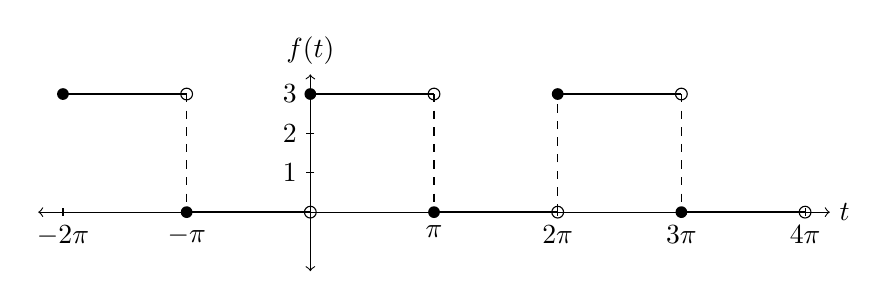
\begin{tikzpicture}[
        scale=0.5, % Updated scale factor to make the figure fit within margins
        % Define a style for the filled circles at the start of steps
        solid_point/.style={circle,fill,inner sep=1.5pt},
        % Define a style for the open circles at the end of steps
        open_point/.style={circle,draw,inner sep=1.5pt}
    ]

    % Define the period
    \def\period{2*pi} % Period is 2*pi

    % Draw the axes
    % Adjusted x-axis range to be from -2.2*pi to 4.2*pi to show periods from -2pi to 4pi
    \draw[<->] (-2.2*pi,0) -- (4.2*pi,0) node[right] {$t$}; % Changed x to t
    % Adjusted y-axis range to accommodate values up to 3
    \draw[<->] (0,-1.5) -- (0,3.5) node[above] {$f(t)$}; % Changed f(x) to f(t)

    % Draw the grid lines for integer multiples of pi
    % Iterates from -2 to 4 to cover the new x-axis range
    \foreach \i in {-2,...,4}
    {
        \pgfmathsetmacro{\xcoord}{\i * pi}
        \draw (\xcoord,0.1) -- (\xcoord,-0.1) node[below] {
            $\ifnum\i=0\else\ifnum\i=1\pi\else\ifnum\i=-1-\pi\else\i\pi\fi\fi\fi$ % Removed 0pi label
        };
    }
    % Draw the grid lines for y-values 1, 2, 3
    \foreach \y in {1,2,3}
        \draw (0.1,\y) -- (-0.1,\y) node[left] {$\y$};

    % Define the step function for one period:
    % f(t) = 3 for 0 <= t < pi
    % f(t) = 0 for pi <= t < 2pi (period is 2pi)

    % Loop to draw multiple periods
    % Changed loop range to draw periods from -2pi to 4pi
    \foreach \k in {-1,0,1} % Draws periods: [-2pi, 0), [0, 2pi), [2pi, 4pi)
    {
        \pgfmathsetmacro{\offset}{\k * \period}

        % First step: value 3 (from offset to offset + pi)
        \draw[thick] (\offset, 3) -- (\offset + pi, 3);
        \node[solid_point] at (\offset, 3) {};
        \node[open_point] at (\offset + pi, 3) {};

        % Second step: value 0 (from offset + pi to offset + 2*pi)
        \draw[thick] (\offset + pi, 0) -- (\offset + \period, 0);
        \node[solid_point] at (\offset + pi, 0) {};
        \node[open_point] at (\offset + \period, 0) {};

        % Add vertical lines to connect steps
        % This connects the open point of the first step (y=3) to the solid point of the second step (y=0)
        \draw[dashed] (\offset + pi, 3) -- (\offset + pi, 0);

        % Connects the open point of the current period's second step (y=0) to the solid point of the next period's first step (y=3)
        % Only draw for the connections between the displayed periods
        \ifnum\k<1 % Adjusted condition to draw lines for k=-1 and k=0
            \draw[dashed] (\offset + \period, 0) -- (\offset + \period, 3);
        \fi
    }

    \end{tikzpicture}
    \caption{A periodic step function} % Added a caption for the figure
    \label{fig:periodic_step_function} % Added a label for cross-referencing
\end{figure}

We will compute the Fourier coefficients $a_0$, $a_n$, and $b_n$ for this function.

\subsubsection{Computing $a_0$}

Recall:
\[
a_0 = \frac{1}{2\pi}\int_0^{2\pi} f(t)\,\mathrm{d}t
\]

For our step function, $f(t) = 3$ for $0 \leq t < \pi$ and $f(t) = 0$ for $\pi \leq t < 2\pi$:
\begin{align*}
a_0 &= \frac{1}{2\pi} \left( \int_0^{\pi} 3\,\mathrm{d}t + \int_{\pi}^{2\pi} 0\,\mathrm{d}t \right) \\
    &= \frac{1}{2\pi} \left( 3\cdot (\pi - 0) + 0 \right) \\
    &= \frac{3\pi}{2\pi}\\
    &= \frac32
\end{align*}

\subsubsection{Computing $a_n$}

Recall:
\[
a_n = \frac{1}{\pi}\int_0^{2\pi} f(t)\cos(nt)\,\mathrm{d}t
\]

Again, split the integral:
\begin{align*}
a_n &= \frac{1}{\pi} \left( \int_0^{\pi} 3\cos(nt)\,\mathrm{d}t + \int_{\pi}^{2\pi} 0\cdot\cos(nt)\,\mathrm{d}t \right) \\
    &= \frac{3}{\pi} \int_0^{\pi} \cos(nt)\,\mathrm{d}t \\
    &= \frac{3}{\pi} \left[ \frac{\sin(nt)}{n} \right]_0^{\pi} \\
    &= \frac{3}{\pi} \left( \frac{\sin(n\pi) - \sin(0)}{n} \right) \\
    &= \frac{3}{\pi} \cdot \frac{0 - 0}{n} \\
    &= 0
\end{align*}

So, all $a_n = 0$ for $n \geq 1$. That is, there are no cosine terms in the Fourier series for this step function. Observing the function graphically, this makes sense because the function is odd about its midpoint.

\subsubsection{Computing $b_n$}

Recall:
\[
b_n = \frac{1}{\pi}\int_0^{2\pi} f(t)\sin(nt)\,\mathrm{d}t
\]

Again, split the integral:
\begin{align*}
b_n &= \frac{1}{\pi} \left( \int_0^{\pi} 3\sin(nt)\,\mathrm{d}t + \int_{\pi}^{2\pi} 0\cdot\sin(nt)\,\mathrm{d}t \right) \\
    &= \frac{3}{\pi} \int_0^{\pi} \sin(nt)\,\mathrm{d}t \\
    &= \frac{3}{\pi} \left[ -\frac{\cos(nt)}{n} \right]_0^{\pi} \\
    &= \frac{3}{\pi} \left( -\frac{\cos(n\pi) - \cos(0)}{n} \right) \\
    &= \frac{3}{\pi} \left( -\frac{(-1)^n - 1}{n} \right) \\
    &= \frac{3}{\pi} \cdot \frac{1 - (-1)^n}{n} \\
    \intertext{Notice that $1 - (-1)^n$ is $0$ for even $n$ and $2$ for odd $n$. Thus, we can express $b_n$ as:}
    b_n &= 
    \begin{cases}
        0 & \text{if $n$ is even} \\
        \frac{6}{n\pi} & \text{if $n$ is odd}
    \end{cases}
\end{align*}


\subsubsection{Summary of Fourier Series}

The Fourier series for this step function is:
\[
f(t) = \frac{3}{2} + \sum_{\substack{n=1 \\ n\ \text{odd}}}^{\infty} \frac{6}{n\pi} \sin(nt)
\]

\subsection{First Few Terms of the Fourier Series Expansion}

\begin{align*}
    \intertext{For $n = 1$, the Fourier approximation is:}
    f_1(t) &= \frac{3}{2} + \frac{6}{\pi} \sin(t) \\[1em]
    \intertext{For $n = 3$, include the next odd term:}
    f_3(t) &= \frac{3}{2} + \frac{6}{\pi} \sin(t) + \frac{2}{\pi} \sin(3t) \\[1em]
    \intertext{For $n = 5$, include up to the fifth term:}
    f_5(t) &= \frac{3}{2} + \frac{6}{\pi} \sin(t) + \frac{2}{\pi} \sin(3t) + \frac{6}{5\pi} \sin(5t)
\end{align*}

These partial sums visualized demonstrate how the Fourier Series converges to the original step function as more terms are added:

\begin{figure}[h!] % Fourier step function and its Fourier approximations
    \centering
    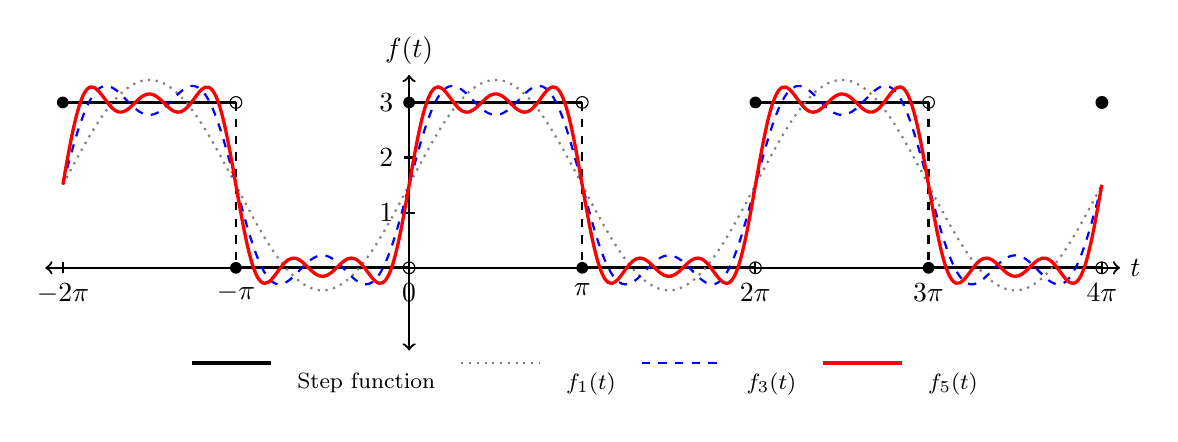
\begin{tikzpicture}[
        scale=0.7,
        solid_point/.style={circle,fill,inner sep=1.5pt},
        open_point/.style={circle,draw,inner sep=1.5pt}
    ]

    % Axes
    \draw[<->,thick] (-6.6,0) -- (12.9,0) node[right] {$t$};
    \draw[<->,thick] (0,-1.5) -- (0,3.5) node[above] {$f(t)$};

    % x-ticks at -2pi, -pi, 0, pi, 2pi, 3pi, 4pi (corrected labels)
    \foreach \i/\label in {-6.28/-2\pi, -3.14/-\pi, 0/0, 3.14/\pi, 6.28/2\pi, 9.42/3\pi, 12.57/4\pi}
        \draw[thick] (\i,0.1) -- (\i,-0.1) node[below] {$\label$};

    % y-ticks at 1, 2, 3
    \foreach \y in {1,2,3}
        \draw[thick] (0.1,\y) -- (-0.1,\y) node[left] {$\y$};

    % Step function: f(t) for -2pi to 4pi
    % Only draw from -2pi (=-6.28) to 4pi (=12.57)
    \foreach \k in {-1,0,1}
    {
        \pgfmathsetmacro{\offset}{\k * 2 * 3.1416}
        % f(t) = 3 for [offset, offset+pi)
        \draw[very thick,black] (\offset,3) -- (\offset+3.1416,3);
        \node[solid_point] at (\offset,3) {};
        \node[open_point] at (\offset+3.1416,3) {};
        % f(t) = 0 for [offset+pi, offset+2pi)
        \draw[very thick,black] (\offset+3.1416,0) -- (\offset+2*3.1416,0);
        \node[solid_point] at (\offset+3.1416,0) {};
        \node[open_point] at (\offset+2*3.1416,0) {};
        % Vertical dashed line
        \draw[dashed,thick] (\offset+3.1416,3) -- (\offset+3.1416,0);
    }
    % Final partial segment if needed to reach exactly 4pi
    \draw[very thick,black] (12.566,3) -- (12.57,3); % 4pi = 12.566, 12.57 for rounding
    \node[solid_point] at (12.566,3) {};
    \node[open_point] at (12.57,3) {};

    % Fourier approximations 
    % f_1(t) - lightest, dotted
    \draw[domain=-6.28:12.57,smooth,samples=300,gray,thick,dotted] plot(\x,{1.5 + (6/3.1416)*sin(deg(\x))});
    % f_3(t) - blue, dashed
    \draw[domain=-6.28:12.57,smooth,samples=300,blue,thick,dashed] plot(\x,{1.5 + (6/3.1416)*sin(deg(\x)) + (2/3.1416)*sin(deg(3*\x))});
    % f_5(t) - heavy, red, solid
    \draw[domain=-6.28:12.57,smooth,samples=300,red,very thick] plot(\x,{1.5 + (6/3.1416)*sin(deg(\x)) + (2/3.1416)*sin(deg(3*\x)) + (6/(5*3.1416))*sin(deg(5*\x))});

    % Legend
    \matrix [row sep=0.2cm, column sep=0.2cm, anchor=north] at (current bounding box.south) {
        \draw[very thick,black] (0,0) -- (1,0); & \node[black] {\footnotesize Step function}; &
        \draw[gray,thick,dotted] (0,0) -- (1,0); & \node[black] {\footnotesize $f_1(t)$}; &
        \draw[blue,thick,dashed] (0,0) -- (1,0); & \node[black] {\footnotesize $f_3(t)$}; &
        \draw[red,very thick] (0,0) -- (1,0); & \node[black] {\footnotesize $f_5(t)$}; \\
    };

    \end{tikzpicture}
    \caption{The periodic step function and its Fourier approximations $f_1(t)$, $f_3(t)$, and $f_5(t)$. Note how the approximation improves as more terms are added.}
    \label{fig:fourier_approximations}
\end{figure}

\section{References}

\begin{itemize}
    \item Khan Academy: \textit{Fourier Series} course.\\
    \url{https://www.khanacademy.org/science/electrical-engineering/ee-signals/ee-fourier-series/v/ee-fourier-series-intro}
\end{itemize}

\end{document}
